% !TEX root = main.tex

\section{搜索}
% Problem solving by search: formalization
% Uninformed search: Breadth-First, Uniform-Cost, Depth-First, Depth-Limited, and Iterative- Deepening
% Properties of search: completeness, optimality, time and space complexity
% Path/cycle checking

搜索主要包括无信息(uninformed)搜索和有信息搜索。
\begin{itemize}
	\item 状态空间(state space)
	\begin{itemize}
		\item 传统搜索:状态空间可见、动作确定性
		\item 非传统搜索:局部搜索、模拟退火、爬坡
	\end{itemize}
	\item 动作(action):不同状态之间的转换
	\item 初始状态(initial state)
	\item 目标/期望(goal)
\end{itemize}
% 对抗搜索(adversarial):博弈树(minimax)、$\alpha-\beta$剪枝

树搜索,边界集(frontier)是未探索的状态集合
\begin{algorithm}[H]
\caption{Tree Search}
\begin{algorithmic}[1]
\Procedure{TreeSearch}{(Frontier, Successors, Goal?)}
\If{Frontier is empty}
\State \Return failure
\EndIf
\State Curr $=$ select state from Frontier
\If{Goal?(Curr)}
\State \Return Curr
\EndIf
\State $\text{Frontier'} = (\text{Frontier} - \{\text{Curr}\}) \cup \text{Successors(Curr)}$
\State \Return TreeSearch(Frontier',Successors,Goal?)
\EndProcedure
\end{algorithmic}
\end{algorithm}

搜索需要关注的几个特性:
\begin{itemize}
	\item 完备性:若解存在,搜索是否总能找到解
	\item 最优性:是否总能找到最小代价的解
	\item 时间复杂性:最大需要被\textemph{生成或展开}\footnote{而不是探索的结点数目}的结点数
	\item 空间复杂性:最大需要被存储在内存中的结点数
\end{itemize}

\subsection{无信息搜索}
无信息搜索并不考虑关于特定搜索问题的领域特定的信息,主要包括宽度优先、一致代价、深度优先、深度受限、迭代加深五种算法。

\subsubsection{宽度优先搜索(BFS)}
将后继加入边界集的\textbf{后面},$b$为最大状态后继数目/分支因子(branching factor),$d$为最短距离解的行动数(注意是\textemph{边数},而不是层数!或者把根节点看作第$0$层也可以)
\begin{itemize}
	\item 完备性与最优性:所有短路总在长路前被探索,某一长度只有有限多条路径,最终可以检测所有长度为$d$的路径,从而找到最优解
	\item 时间复杂度:$1+b+b^2+\cdots+b^d+(b^d-1)b=O(b^{d+1})$,最差情况在最后一层的最后一个节点才探索到最优解,从而前面$b$个节点都要展开第$d+1$层
	\item 空间复杂度:$b(b^d-1)=O(b^{d+1})$,需要将边界集都存储下来,同上最后一层
\end{itemize}

\subsubsection{深度优先搜索(DFS)}
将后继加入边界集的\textbf{前面},即总是展开边界集中最深的节点
\begin{itemize}
	\item 完备性
	\begin{itemize}
		\item 无限状态空间:不能保证
		\item 有限状态空间无限路径:不能保证(可能有环)
		\item 有限状态空间+路径/重复状态剪枝:可以保证
	\end{itemize}
	\item 最优性:因完备性不能保证,故最优性也不能保证
	\item 时间复杂性:$O(b^m)$,其中$m$为状态空间的最长路的长度(若$m>>d$,则非常糟糕;但如果有大量解路径,则会快于BFS)
	\item 空间复杂性:$O(bm)$,\textbf{线性空间复杂性}是DFS最大的优点。边界集只包含当前路径的最深节点以及回溯节点(backtrack points为当前路径上节点的未探索的兄弟sibling)。
	注意这里需要记录路径上每个结点的孩子,因已被扩展。
\end{itemize}

\subsubsection{一致代价(Uniform-cost)}
一致代价搜索(Uniform cost search, UCS)\footnote{至于为什么叫Uniform,可以看\url{https://math.stackexchange.com/questions/112734/in-what-sense-is-uniform-cost-search-uniform}和\url{https://cs.stackexchange.com/questions/6072/why-is-uniform-cost-search-called-uniform-cost-search},比较合理的解释是到达同一结点的cost都被认为是相同的(寻找最优解时)。一致的算法总是选择边界集中第一个元素。}的边界集以路径开销升序排序,总是先展开最低开销的路径。
如果每一个动作都是一样的代价,则一致代价等价于BFS。
\begin{itemize}
	\item 完备性与最优性:假设所有转移都有代价$\geq\eps>0$,所有更低代价的路径都在高代价路径之前被展开,只有有限多的路径开销小于最优解的开销,故最终一定会到达最优解
	\item 时间复杂性:$O(b^{\lfloor C^\star/\eps\rfloor+1})$,对应着BFS中$d=C^\star/\eps$,其中$C^\star$为最优解的开销,最坏情况就是每一层开销都很小为$\eps$,那么需要$\lfloor C^\star/\eps\rfloor$层
	\item 空间复杂性:$O(b^{\lfloor C^\star/\eps\rfloor+1})$
\end{itemize}
\begin{figure}[H]
\centering
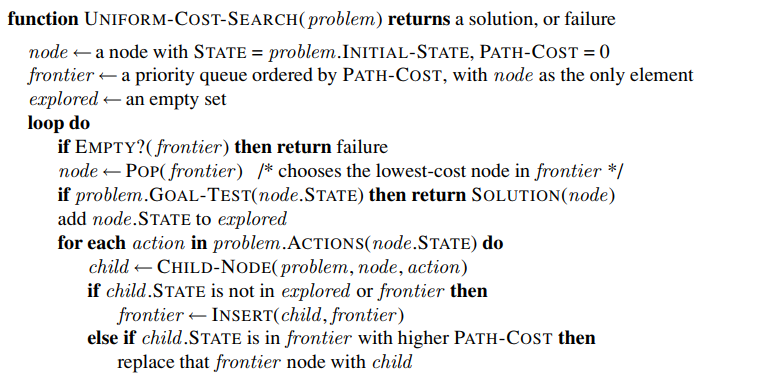
\includegraphics[width=0.7\linewidth]{fig/UCS.png}
\end{figure}
注意算法中几个关键点:从队列Pop出一个结点后
\begin{enumerate}
	\item \textemph{先做目标检测},如果是目标则立即返回(也就是说要扩展完结点进入下一层才会触发解返回)
	\item 将结点状态标记为\textemph{已探索(explored)},然后扩展(expand)该结点
	\item 做环检测,如果孩子\textemph{不在\underline{已探索或边界集}中},将孩子节点加入边界集
	\item 如果孩子在边界集中且有更高的路径开销,则将边界集中的结点用孩子结点进行\textemph{替换}
\end{enumerate}

\subsubsection{深度受限搜索(Depth-limited)}
只在最大深度执行DFS,因此无穷路径长不会存在问题
\begin{itemize}
	\item 完备性与最优性:不能保证,若解的深度大于$L$
	\item 时间复杂度:$O(b^L)$
	\item 空间复杂度:$O(bL)$
\end{itemize}

\subsubsection{迭代加深搜索(Iterative Deepening)}
IDS逐渐增加最大深度$L$,对每一个$L$做深度受限搜索
\begin{itemize}
	\item 完备性:可以保证
	\item 最优性:如果开销一致\footnote{若开销不一致,则可以采用代价界(cost bound)来代替:仅仅展开那些路径开销小于代价界的路径,同时要记录每一层深搜的最小代价。这种方式的搜索开销会非常大,有多少种不同路径开销就需要多少次迭代循环。},则可以保证
	\item 时间复杂性:$(d+1)b^0+db+(d-1)b^2+\cdots+b^d=O(b^d)$,第$0$层搜了$(d+1)$次,以此类推。可以看到时间复杂度是\textbf{比BFS优}的,因为最后一层的结点并未进行展开。
	\item 空间复杂性:$O(bd)$,同DFS
\end{itemize}

\subsubsection{双向搜索(Bidirectional)}
从源结点和汇结点同时采用BFS,直到两个方向的搜索汇聚到中间。
\begin{itemize}
	\item 完备性:由BFS保证
	\item 最优性:若一致代价则可保证
	\item 时间复杂性:$O(b^{d/2})$
	\item 空间复杂性:$O(b^{d/2})$
\end{itemize}

\subsubsection{环路/路径检测}
所有检测都是在\textemph{扩展时}进行:
\begin{itemize}
	\item 环路(cycle)检测:检测当前状态是否与所有已探索的(explored)状态重复(BFS)
	\item 路径(path)检测:只检测当前状态是否与该路径上的状态重复(DFS)
\end{itemize}
注意不能将环路检测运用在BFS上,因为这会破坏其空间复杂度的优势。

环路检测运用到UCS上依然\textemph{可以保证最优性}\footnote{注意这在启发式搜索中不一定成立}。
因为UCS第一次\textemph{探索}(注意不是展开)到某一状态的时候已经发现最小代价路径,因而再次探索该状态不会发现路径比原有的更小。

\subsubsection{总结}
\begin{center}
\begin{tabular}{ccccccc}\hline
& BFS & UCS & DFS & Depth-limited & IDS & Bidirectional\\\hline
完备性 & \cmark & \cmark & \xmark & \xmark & \cmark & \cmark\\
时间复杂度 & $O(b^d)$ & $O(b^{\lfloor C^\star/\eps\rfloor+1})$ & $O(b^m)$ & $O(b^l)$ & $O(b^d)$ & $O(b^{d/2})$\\
空间复杂度 & $O(b^d)$ & $O(b^{\lfloor C^\star/\eps\rfloor+1})$ & $O(bm)$ & $O(bl)$ & $O(bd)$ & $O(b^{d/2})$\\ 
最优性 & \cmark & \cmark & \xmark & \xmark & \cmark & \cmark\\\hline
\end{tabular}
\end{center}

\begin{example}
$N$个传教士和$N$个食人族要过河,他们都在河的左岸。
现在只有一条船能够运载$K$个人,要把他们都运往右岸。
要满足无论何时何地,传教士的数目都得大于等于食人族的数目,或者传教士数目为0。
\end{example}
\begin{analysis}
考虑对问题形式化为搜索问题
\begin{itemize}
	\item 状态$(M,C,B)$,其中$M$为左岸传教士数目,$C$为左岸食人族数目,$B=1$指船在左岸
	\item 动作$(m,c)$指运$m$个传教士和$c$个食人族到对岸
	\item 先决条件:传教士数目和食人族数目满足限制
	\item 效果:$(M,C,1)\stackrel{(m,c)}{\implies}(M-m,C-c,0)$\\
	$(M,C,0)\stackrel{(m,c)}{\implies}(M+m,C+c,1)$
\end{itemize}
\end{analysis}